\chapter{Background and Related Work}
\label{chap:background}

\begin{introduction}

Before diving into the work done in Resilient \ac{fl}, it is essential to understand concepts related to \ac{ml}, going from centralized to distributed \ac{ml}, and understand how \ac{fl} fits in the distributed \ac{ml} landscape. Given the distributed nature of \ac{fl}, it is also essential to analyze the communication protocols that can be used in this context. 

This aims to show that \ac{fl} is a compelling solution for training \ac{ml} models in a collaborative manner, while preserving data privacy. However, its success relies on the robustness of the learning and communication layers, especially in heterogeneous environments, where devices have different capabilities and can enter or leave the network anytime.

To address these challenges, this chapter transitions to the state-of-the-art in \ac{fl} research, focusing on resilient approaches and other \ac{fl} frameworks that attempt to address the challenges of dynamic networks and unreliable devices, while highlighting their main strengths, limitations, and contributions. These insights are essential for developing the proposed solution, as they provide a solid foundation to identify the gaps and requirements.

\end{introduction}


\section{Centralized Machine Learning}
\label{sec:centralized-ml}

Centralized \ac{ml} is the most widely used approach in the field of \ac{ai}, where a single entity collects all the data, processes it and trains a \ac{ml} model \cite{abdulrahman2020survey}. This data can be collected from multiple sources, including sensors, databases, and other devices. 

The \ac{ml} process can be divided into three main categories: supervised learning, unsupervised learning, and reinforcement learning \cite{sahoo2024evolution}, each with its own characteristics and applications as shown in Figure \ref{fig:ml_types}.

\begin{figure}[ht]
    \centering
    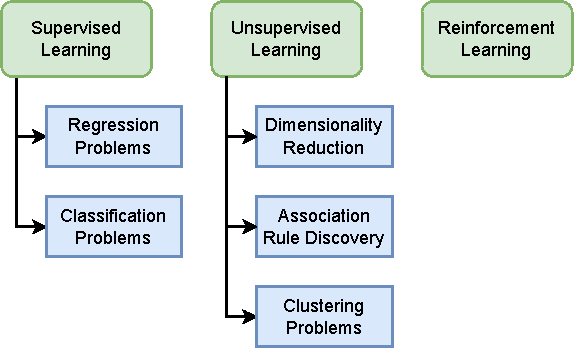
\includegraphics[width=0.7\textwidth]{figs/ml_types.pdf}
    \caption[Overview of \ac{ml} Learning Paradigms]{Comprehensive taxonomy of \ac{ml}, detailing its three fundamental learning paradigms: Supervised Learning, Unsupervised Learning, and Reinforcement Learning, and their associated problem domains.}
    \label{fig:ml_types}
\end{figure}

Supervised learning is used when the data is labeled, and the goal is to predict the output based on the input data. This type of learning is used in classification problems, where the output is a category, and regression problems, where the output is a continuous value. 

Unsupervised learning is used when the data is not labeled and the goal is to find patterns in it. This is used in clustering problems, where the goal is to group similar data points together, association rule discovery problems, where the goal is to find relationships between variables, and dimensionality reduction problems, where the goal is to reduce the number of variables in the data.

Finally, reinforcement learning is used when the agent learns to interact with the environment by taking actions and receiving rewards. The goal is to learn a policy that maximizes the cumulative reward.

Given that the data is centralized, the training process can be done on a single machine, without the need for communication between different entities. This makes the training process easier to implement, monitor, and resource-efficient. However, it also has some drawbacks, such as privacy concerns when the data is sensitive or confidential, a single point of failure, and scalability issues when the data or the model is too large to be computed by a single machine.

\subsection{Neural Networks}
\label{sec:neural-networks}

\ac{nn} represent a fundamental and powerful class of models in \ac{ml}, particularly central to the field of deep learning. While centralized \ac{ml} can employ various model types, \acp{nn} are frequently used due to their ability to learn complex patterns.

A \ac{nn} is structured in layers, typically including an input layer, one or more hidden layers, and an output layer. Each layer consists of interconnected nodes (or neurons), with connections having associated weights and biases. During training, data passes through the \ac{nn} (forward pass), and calculations are performed at each neuron using activation functions, resulting in a prediction. The difference between the prediction and the actual target is quantified by a loss function. 

To minimize this loss, the \ac{nn} is trained using algorithms like backpropagation \cite{rumelhart1986learning}, which calculates the gradients of the loss function concerning the \ac{nn}'s weights and biases. These gradients indicate the direction and magnitude of the change needed for each weight and bias to reduce the loss. Various optimization methods (e.g., Gradient Descent, Adam \cite{kingma2014adam}) then use these gradients to update the weights and biases, iteratively improving the model's performance. 

A simple representation of an \ac{nn} structure is shown in Figure \ref{fig:nn_structure}. The input layer receives the data, the hidden layers process it, and the output layer produces the final prediction. Each connection between neurons has a weight that determines its influence on the output.

\begin{figure}[!htb]
    \centering
    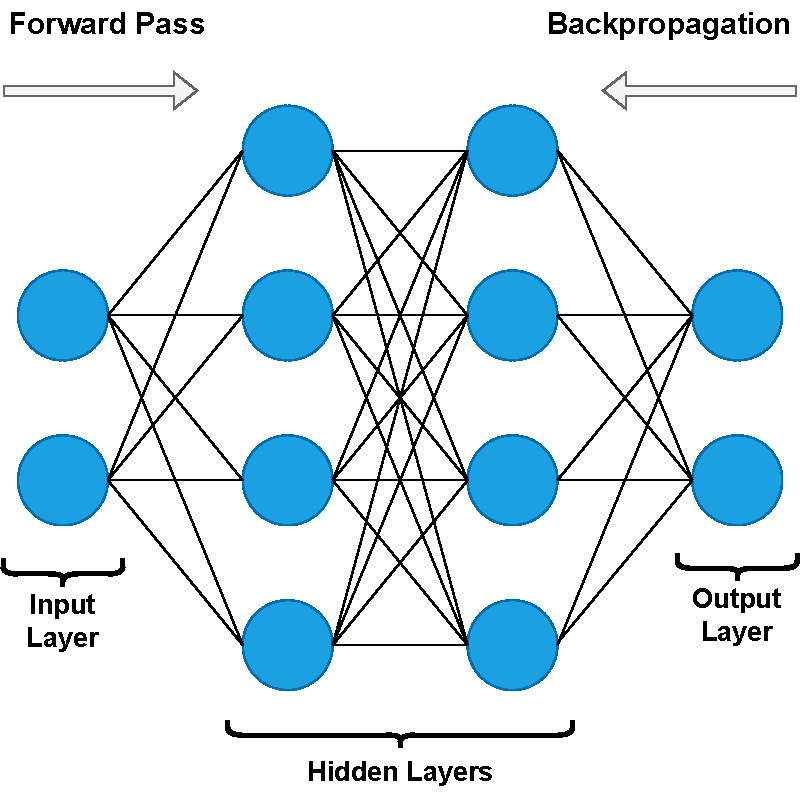
\includegraphics[width=0.6\textwidth]{figs/nn_structure.pdf}
    \caption[Neural Network Structure]{Structure of a typical Neural Network, detailing its Input, Hidden, and Output Layers. The diagram highlights the directional flow of computation during the Forward Pass and the gradient-based optimization process of Backpropagation.}
    \label{fig:nn_structure}
\end{figure}

In the context of distributed and \ac{fl}, the model being trained is often a \ac{nn}. It is crucial to distinguish this model network structure from the communication network of interconnected devices (workers and servers) participating in the distributed learning process. For the remainder of this dissertation, we use the term Model to refer specifically to a \ac{nn}, and Network to denote a communication network, unless otherwise stated.



\section{Distributed Machine Learning}
\label{sec:distributed-ml}

Distributed \ac{ml} is an approach where the data or model is distributed across multiple machines and the training process is done in a distributed manner that, under certain conditions, enables faster training and allows larger models and datasets that can't be processed by a single machine \cite{10410765, 10608461}. 

The distributed training process can follow different architectures and techniques. In \cite{9120226}, the authors present a taxonomy that classifies distributed \ac{ml} into three categories: Model vs Data Parallelism, Centralized vs Decentralized Optimization, and Synchronous vs Asynchronous Scheduling.

\subsection{Model vs Data Parallelism}
\label{sec:model-vs-data-parallelism}

Model and Data Parallelism are two different strategies for distributing large workloads, one maps the model to multiple machines, and the other maps the data to multiple machines.

Model parallelism involves dividing a \ac{ml} model into partitions to be processed by different machines, and it is particularly beneficial when the model is too large to fit in memory. This partitioning can be done in two ways: vertical partitioning, which splits the model between layers, or horizontal partitioning, which divides individual layers as shown in Figure \ref{fig:model_parallelism}.

\begin{figure}[!htb]
    \centering
    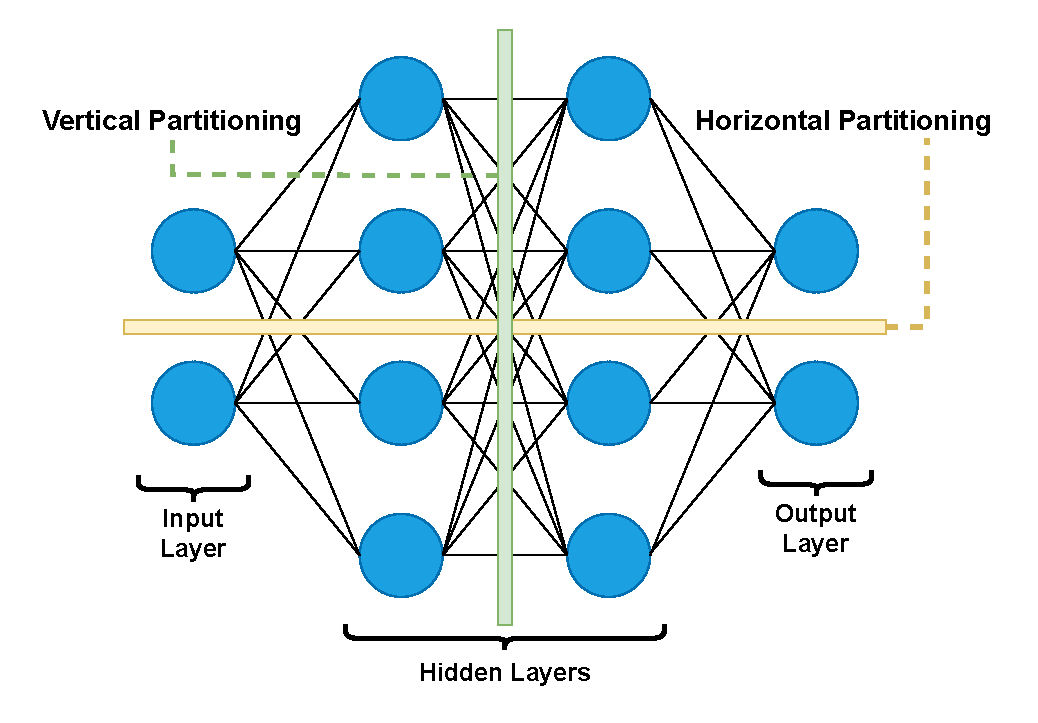
\includegraphics[width=0.7\textwidth]{figs/model_parallelism.pdf}
    \caption[Model Parallelism Partitioning]{Illustration of Model Parallelism, distinguishing between Vertical Partitioning, where the model is split across layers, and Horizontal Partitioning, where individual layers are divided across multiple machines.}
    \label{fig:model_parallelism}
\end{figure}

Vertical partitioning is simpler to implement since it requires transporting intermediate outputs (activations) between machines. On the other hand, horizontal partitioning, which splits the layers themselves, is more complex because it requires managing numerous inter-machine connections.

In data parallelism, multiple machines process different subsets of the data using the same model architecture. This approach aggregates gradients or weights from various machines to update the model parameters, facilitating parallelized computation. The communication overhead and scalability depend on the model size and the efficiency of the aggregation mechanism. Data parallelism is often easier to implement and scale than model parallelism, allows data privacy when combined with privacy-preserving techniques, and is widely adopted in distributed systems.

\subsection{Centralized vs Decentralized Optimization}
\label{sec:centralized-vs-decentralized-optimization}

In centralized optimization, a central server (parameter server) aggregates gradients computed by distributed workers and updates the global model parameters. While this architecture simplifies the synchronization and coordination of workers, it can become a bottleneck in large clusters due to communication overhead and reliance on a single server for updates, because the gradients are sent to the parameter server after each batch, and the updated weights are sent back to the workers. Advanced implementations mitigate these issues by distributing the parameter server role across multiple nodes. Figure \ref{fig:centralized_opt} shows the centralized optimization process.

\begin{figure}[!htb]
    \centering
    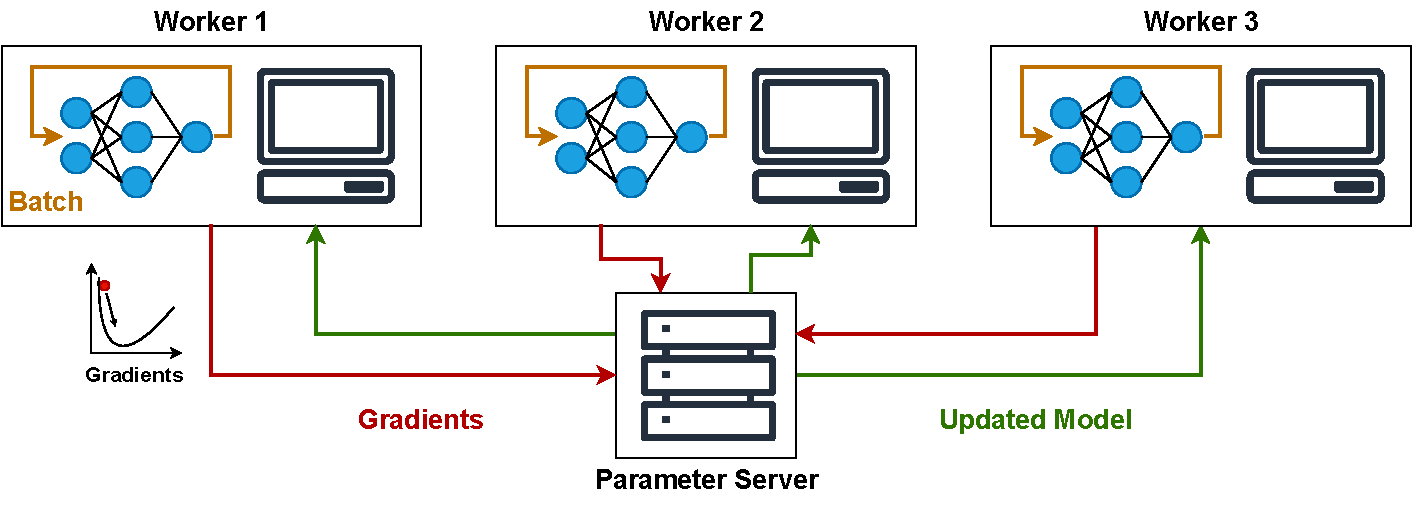
\includegraphics[width=\textwidth]{figs/centralized_opt.pdf}
    \caption[Centralized Optimization Process]{Diagram illustrating the Centralized Optimization process, where multiple Workers compute gradients and send them to a single Parameter Server, which then aggregates these gradients to update the global model and sends the Updated Model back to the workers.}
    \label{fig:centralized_opt}
\end{figure}

Decentralized optimization involves each worker training its local model independently, periodically synchronizing with peers or a master node (parameter server) by sending the weights. This method can reduce dependency on a central server, enabling higher scalability and tolerance to communication delays. However, ensuring convergence and minimizing inconsistencies among workers requires careful tuning of synchronization strategies and hyperparameters. Figure \ref{fig:decentralized_opt} shows the decentralized optimization process.

\begin{figure}[!htb]
    \centering
    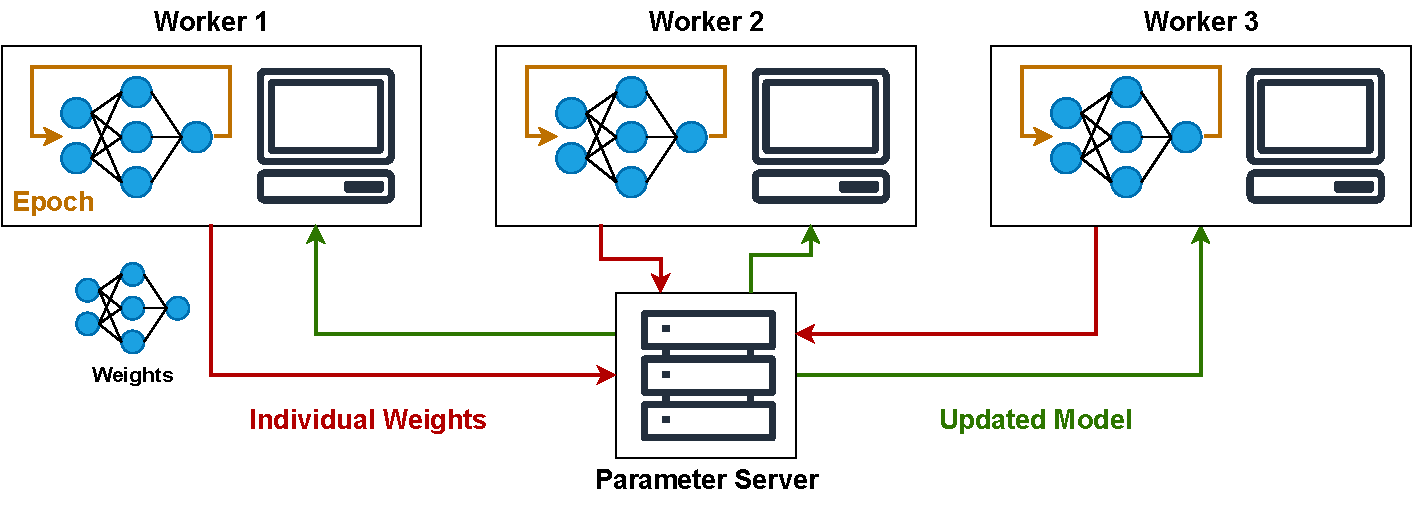
\includegraphics[width=\textwidth]{figs/decentralized_opt.pdf}
    \caption[Decentralized Optimization Process]{Diagram illustrating the decentralized optimization process, where workers train their local models independently and periodically synchronize with a parameter server by exchanging individual weights and receiving updated models.}
    \label{fig:decentralized_opt}
\end{figure}

These two approaches can then be used together or individually in a hierarchical manner \cite{liu2020client}, where the workers are divided into groups, each group has a master node, and the parameter server aggregates the gradients or weights from the master nodes. This approach can reduce the communication overhead and improve the system's scalability.

\subsection{Synchronous vs Asynchronous Scheduling}
\label{sec:synchronous-vs-asynchronous-scheduling}

In synchronous systems, workers operate in lockstep, aggregating all updates before proceeding to the next training iteration. This approach minimizes inconsistencies among workers and is easier to implement and debug, but it can lead to resource underutilization due to waiting for slower nodes (stragglers). Model aggregation in synchronous systems typically uses weighted averaging, where each worker's update is scaled based on factors such as data size or importance before being combined into a global model.

The weighted averaging is defined as follows:
\begin{equation}
    \theta_{t+1} = \frac{\sum_{i=1}^{N} w_i \cdot \theta_i}{\sum_{i=1}^{N} w_i}
\end{equation}

where $\theta_{t+1}$ is the updated model parameters, $N$ is the number of workers, $w_i$ is the weight assigned to worker $i$, and $\theta_i$ is the model parameters from worker $i$. The weights are typically proportional to each worker’s data size or reliability. The normalization ensures that the update is a true weighted average, maintaining scale consistency and promoting a balanced aggregation.


Asynchronous systems allow workers to proceed with their computations independently, updating the model parameters as they complete their tasks. While this maximizes resource utilization and can be more scalable, it introduces challenges such as stale updates, which can slow convergence or degrade model performance. To mitigate this, linear interpolation is often used for model aggregation, blending new updates with the current model state to maintain stability. These complexities make asynchronous systems harder to implement and debug, but potentially more efficient in heterogeneous environments.

The linear interpolation is defined as follows:
\begin{equation}
    \theta_{t+1} = \theta_t + \alpha \cdot (\theta_i - \theta_t)
\end{equation}

where $\theta_{t+1}$ is the updated model parameters, $\theta_t$ is the current model parameters, $\alpha$ is the interpolation factor (0 < $\alpha$ < 1), and $\theta_i$ is the model parameters from worker $i$. This allows the system to blend new updates with the current model state, maintaining stability while incorporating fresh information.



\section{Federated Learning}
\label{sec:federated-learning}

\ac{fl} is a paradigm of distributed \ac{ml},  which can differ from other distributed \ac{ml} approaches in three ways \cite{liu2022distributed}. First, the data cannot be shared between the devices, ensuring privacy, security, and ownership. This way, laws and regulations such as the \ac{gdpr} are easier to comply with. Second, \ac{fl} is designed to work in a distributed manner, while maximizing resource utilization, allowing organizations to collaborate without sharing data. Finally, \ac{fl} can have security mechanisms such as encryption to further protect the data.

The core process of \ac{fl}, where training is coordinated across multiple devices while keeping data local, is illustrated in Figure \ref{fig:fl_process}. 

\begin{figure}[!htb]
    \centering
    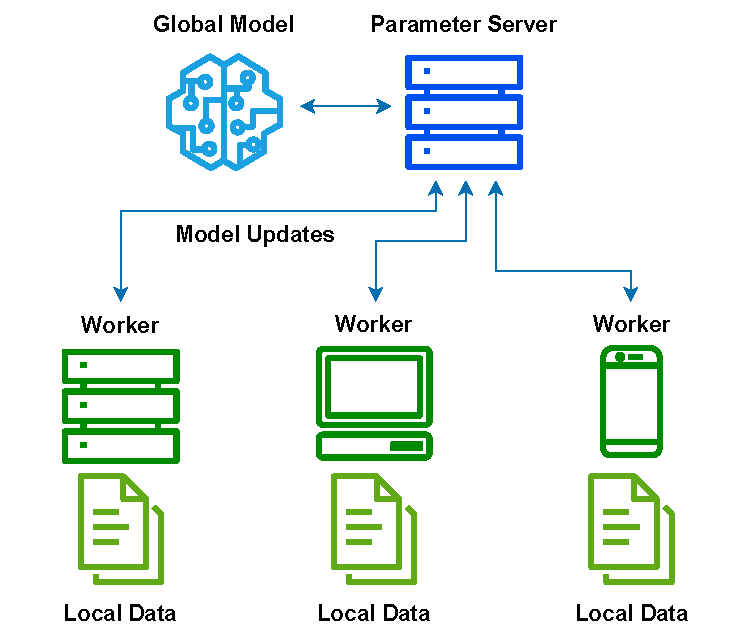
\includegraphics[width=0.7\textwidth]{figs/fl_process.pdf}
    \caption[Federated Learning Process Overview]{The core process of Federated Learning, illustrating how a central Parameter Server coordinates model training across multiple Workers, where each Data remains stored locally, ensuring privacy and security by only exchanging Model Updates for a Global Model.}
    \label{fig:fl_process}
\end{figure}

\ac{fl} can be divided into three main categories: horizontal \ac{fl}, vertical \ac{fl} and federated transfer learning \cite{yang2019federated}. Horizontal \ac{fl} is applicable when the datasets of participating entities share the same feature space but have different samples \cite{yang2020horizontal}. Vertical \ac{fl} is used when the datasets share the same samples but have different features \cite{liu2024vertical}. Federated transfer learning is used when the datasets have different feature spaces and samples, and the goal is to transfer knowledge from one dataset to another \cite{saha2021federated}.

Most of the \ac{fl} use cases are related to mobile devices, industrial engineering, and healthcare, where the data is sensitive and cannot be shared, or the centralized approach is not feasible due to the large amount of data \cite{li2020review}. When these restrictions do not apply, the other approaches might be more suitable.

\section{Communication Protocols}
\label{sec:communication-protocols}

\ac{fl} relies on efficient communication protocols to manage distributed training, ensuring privacy, scalability, and minimal overhead. The protocol choice depends on the system requirements, such as the number of devices, network conditions, and security constraints. This section evaluates the scalability, fault tolerance, security, and suitability for \ac{fl} applications of four prominent communication protocols: \ac{mpi} \cite{gabriel2004open}, \ac{mqtt} \cite{light2017mosquitto}, Kafka \cite{kreps2011kafka}, and Zenoh \cite{corsaro2023zenoh}, while highlighting their key features and limitations.

\subsection{MPI}
\label{sec:mpi}

\ac{mpi} is a widely used communication protocol in \ac{hpc} environments, providing low-latency, high-throughput communication between nodes, because it is designed to handle the message-passing paradigm with explicit exchange of data by send and receive operations. 

However, \ac{mpi} relies on static configurations, requiring predefined communication endpoints and also lacks built-in support for fault tolerance, making it unsuitable for handling worker disconnections or failures, which are common in real-world \ac{fl} systems. 

While its synchronous communication model ensures consistency, it introduces constraints that hinder scalability in flexible, decentralized training scenarios. Additionally, \ac{mpi} does not provide native support for encryption or authentication, relying instead on secure underlying transport layers like \ac{ssh} or network-level security configurations.

Figure \ref{fig:mpi_comm} illustrates the basic communication flow in an \ac{mpi} system, where processes exchange messages explicitly.

\begin{figure}[!htb]
    \centering
    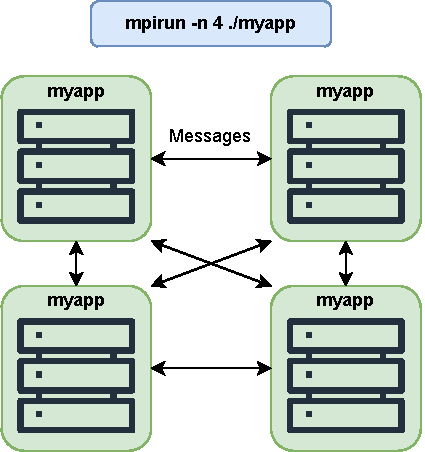
\includegraphics[width=0.45\textwidth]{figs/mpi_comm.pdf}
    \caption[MPI Communication Flow]{The communication flow within an \ac{mpi} system, showing four interconnected application processes. This setup relies on a static configuration, where the number of workers is fixed and new participants cannot dynamically join, with all processes typically executing the same program.}
    \label{fig:mpi_comm}
\end{figure}

\subsection{MQTT}
\label{sec:mqtt}

\ac{mqtt} is a lightweight publish-subscribe protocol designed for resource-constrained devices and low-bandwidth networks. It employs a centralized broker to mediate client communication, allowing devices to dynamically join or leave the system without disrupting operations, making it appealing for \ac{fl} use cases. 

It also offers a native way to notify clients when other clients disconnect, which is helpful for \ac{fl} systems where worker availability may fluctuate. Despite its advantages for edge deployments, this centralized architecture can become a bottleneck in large-scale deployments, particularly as the volume of exchanged model updates increases. 

\ac{mqtt} supports \ac{tls} and \ac{mtls} for secure communication on top of \ac{tcp}, with client authentication and role-based access control. However, the dependence on a broker limits scalability compared to fully decentralized protocols.

Figure \ref{fig:mqtt_comm} illustrates the communication flow in an \ac{mqtt} system, where clients publish messages to topics and subscribe to receive updates.

\begin{figure}[!htb]
    \centering
    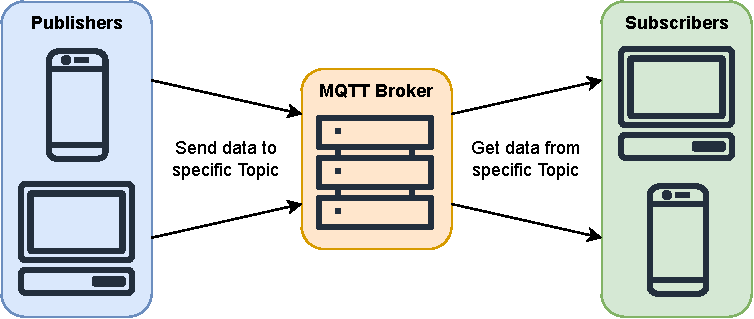
\includegraphics[width=0.75\textwidth]{figs/mqtt_comm.pdf}
    \caption[MQTT Communication Flow]{Illustration of the \ac{mqtt} communication flow, showcasing the publish-subscribe model. Publishers send data to a central \ac{mqtt} Broker, which then mediates the distribution of messages to relevant Subscribers based on specific topics.}
    \label{fig:mqtt_comm}
\end{figure}

\subsection{Kafka}
\label{sec:kafka}

Kafka is a distributed streaming platform optimized for real-time data processing. Its publish-subscribe model supports dynamic and large-scale systems, offering persistent storage and robust fault tolerance through distributed broker clusters. 

However, Kafka's suitability for \ac{fl} is hindered by the latency introduced through its brokered communication model, where the additional communication hops required for routing messages through brokers can slow down the synchronization of model updates, which is critical in iterative training processes. 

The only native disconnection notification mechanism is inspection of connected groups. To participate in a group, clients must subscribe with the same group ID, but this approach adds considerable overhead because when a client joins or leaves, partitions must be rebalanced, which can be time-consuming and resource-intensive.

Similarly to \ac{mqtt}, Kafka supports \ac{tls}, \ac{mtls}, client authentication, and role-based access control for secure communication.

Figure \ref{fig:kafka_comm} illustrates the communication flow in a Kafka system, where producers publish messages to topics and consumers subscribe to receive updates.

\begin{figure}[!htb]
    \centering
    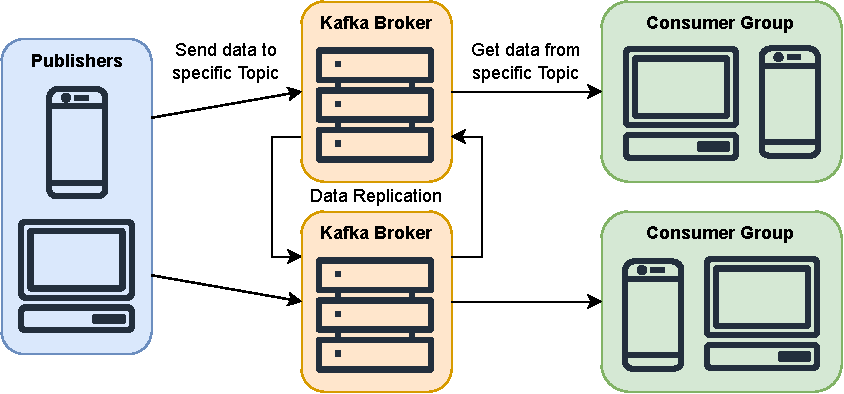
\includegraphics[width=0.9\textwidth]{figs/kafka_comm.pdf}
    \caption[Kafka Communication Flow]{Illustration of the Kafka communication flow, detailing how Publishers send data to topics managed by a distributed Kafka Broker cluster. This system leverages data replication for persistence and fault tolerance, and messages are consumed by organized Consumer Groups from specific topics.}
    \label{fig:kafka_comm}
\end{figure}

\subsection{Zenoh}
\label{sec:zenoh}

Zenoh is a decentralized communication middleware specifically designed for dynamic and resource-constrained environments. Unlike broker-based protocols, Zenoh adopts a fully decentralized architecture that eliminates single points of failure and enables seamless communication among devices, even in unreliable network conditions. 

Similar to \ac{mqtt}, it offers a native way that allows participants to be notified when other participants leave the network without needing a centralized broker.

It supports multiple communication methods, including \ac{tcp}, \ac{tls} and \ac{mtls}, allowing devices to adapt to varying security and performance requirements. Zenoh also supports the use of \acp{acl}, enabling fine-grained permission management to control which entities can publish or subscribe to specific data. Despite its advantages, Zenoh is a relatively new protocol with a less mature ecosystem compared to established solutions such as the ones mentioned above, which may limit its adoption in existing \ac{fl} systems.

Figure \ref{fig:zenoh_comm} illustrates the communication flow in a Zenoh system, where devices communicate directly without a central broker and can join or leave the network dynamically.

\begin{figure}[!htb]
    \centering
    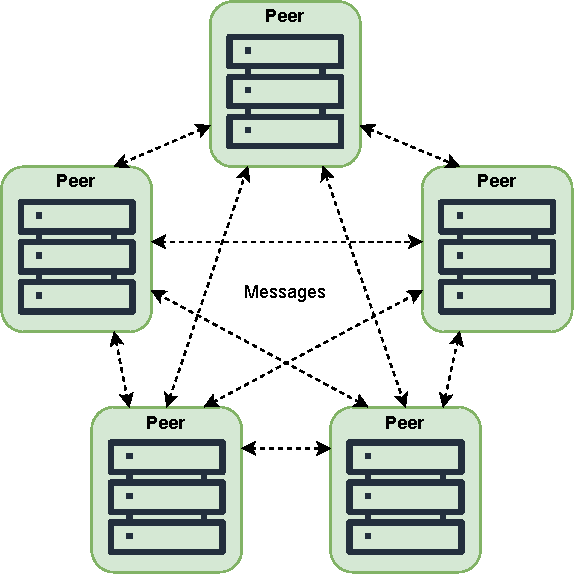
\includegraphics[width=0.6\textwidth]{figs/zenoh_comm.pdf}
    \caption[Zenoh Communication Flow]{Illustration of the Zenoh communication flow, highlighting its fully decentralized peer-to-peer architecture. This design allows individual Peers to communicate directly and dynamically join or leave the network at any moment without requiring a central broker. Adapted from Zenoh Documentation.}
    \label{fig:zenoh_comm}
\end{figure}


\subsection{Summary of Communication Protocols}

Communication protocols are critical to enable efficient, secure, and scalable \ac{fl} systems. Each protocol discussed offers unique strengths and limitations, making them suitable for different scenarios. The choice of protocol should be based on the specific requirements of the \ac{fl} system, such as the number of devices, network conditions, and security constraints, to ensure optimal performance and reliability.

Table~\ref{tab:communication_protocols} summarizes the communication protocols' main features, highlighting their suitability for our scenario.

\begin{table}[!htb]
    \caption[Comparative Analysis of FL Communication Protocols]{A comparative analysis of communication protocols, including \ac{mpi}, \ac{mqtt}, Kafka, and Zenoh, detailing their characteristics in terms of scalability, fault tolerance, security, and general suitability for \ac{fl} deployments.}
    \label{tab:communication_protocols}
    \centering
    \begin{tabular}{Sc Sc Sc Sc Sc}
    \toprule
    \textbf{Protocol} & \textbf{Scalability} & \textbf{Fault Tolerance} & \textbf{Security} & \textbf{Suitability} \\
    \midrule
    \ac{mpi}  & 
        Limited &
        \begin{tabular}[c]{@{}c@{}}No built-in\\support\end{tabular} & 
        Relies on \ac{ssh} & 
        \begin{tabular}[c]{@{}c@{}}Low, lacks fault\\tolerance and scalability\end{tabular} \\
    \ac{mqtt} & 
        Moderate &
        Moderate &
        \begin{tabular}[c]{@{}c@{}}\ac{tls}, \ac{mtls}\\role-based\end{tabular} &
        \begin{tabular}[c]{@{}c@{}}High, suitable when\\using a central broker\end{tabular} \\
    Kafka & 
        High &
        High &
        \begin{tabular}[c]{@{}c@{}}\ac{tls}, \ac{mtls}\\role-based\end{tabular} &
        \begin{tabular}[c]{@{}c@{}}Moderate, latency can\\hinder synchronization\end{tabular} \\
    Zenoh & 
        High &
        High &
        \begin{tabular}[c]{@{}c@{}}\ac{tls}, \ac{mtls}\\\ac{acl}\end{tabular} &
        \begin{tabular}[c]{@{}c@{}}High, but limited\\ecosystem maturity\end{tabular} \\
    \bottomrule
\end{tabular}
\end{table}

In our case, a centralized server (parameter server) coordinates the training process, and the system is designed to be resilient to worker disconnections. This means that a centralized communication broker such as \ac{mqtt} is not a problem, and the system can benefit from its lightweight nature. However, \ac{mpi} is unsuitable for our system because it is designed for static configurations.



\section{Systematic Literature Review}
\label{sec:slr}

The state-of-the-art in \ac{fl} is vast and diverse; however, studies focusing on the type of resilience for this work are harder to find. To address this challenge, a systematic literature review was conducted.

The first step in the review process was to define the research questions that will guide the search for relevant literature. The following questions were defined:

\begin{itemize}
    \item \textbf{RQ1:} How can Federated Learning frameworks be designed to ensure robustness against node failures across dynamic network environments?
    \item \textbf{RQ2:} What communication layer architectures are most suitable for supporting fault-tolerant and resilient Federated Learning under dynamic network conditions?
\end{itemize}

The first research question aims to understand the strategies and mechanisms that can be used to improve the robustness of \ac{fl} frameworks, while the second question focuses on the communication layer, which is a critical component for the success of \ac{fl} in dynamic networks. These questions aim to identify keywords and concepts that can be used to search for relevant literature.

The next step was to define the queries that would be used to search for relevant literature in databases, specifically SCOPUS. To narrow the search and improve the quality of the results, only records from journals and conferences published in the last five years were considered.

Keywords such as ''Federated Learning'', ''Resilience'', ''Communication'' and ''Fault Tolerance'' emerge from the research questions, but some challenges remain to be addressed. 

For instance, the term ''Resilience'' in \ac{fl} is primarily used in the context of attacks, data poisoning, and to ensure that the \ac{ml} models converge. With the term ''Communication'', most of the results are related to papers focusing on communication costs, communication efficiency, or just an analysis of the communication layer, not including fault tolerance to node failures or network delays. 

Therefore, the query with the most relevant results was: TITLE-ABS-KEY ( ''federated learning'' ) AND TITLE-ABS-KEY ( ''fault tole*'' ).

The review process, as shown in Figure~\ref{fig:prisma}, started with retrieving 121 records from SCOPUS using the previously defined query and filters. This step was conducted on October 31, 2024.

\begin{figure}[!htb]
    \centering
    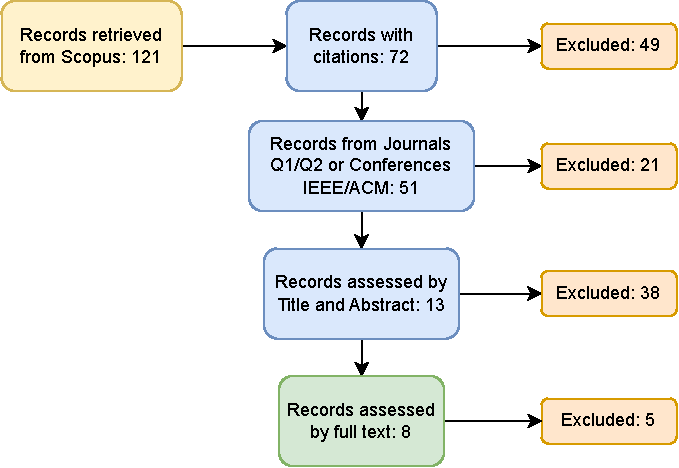
\includegraphics[width=0.8\textwidth]{figs/prisma.pdf}
    \caption[Systematic Literature Review Process]{Detailed flow of the systematic literature review process, beginning with 121 retrieved records from SCOPUS. The diagram illustrates five sequential exclusion steps that systematically filtered irrelevant studies, culminating in a final set of 8 relevant records for in-depth analysis.}
    \label{fig:prisma}
\end{figure}

Studies without citations were excluded from these records to focus on work that has had an observable impact on the research community. This step reduced the pool to 72 records, excluding 49 records.

Given the proven quality and reputation of Journals Q1 and Q2 and Conferences IEEE and ACM, only records from these sources were considered, where 51 records were selected and 21 were excluded.

The next step was to screen the records by title and abstract, to identify studies relevant to the research questions, namely those that focus on fault tolerance of node failures and communication layer architectures. This step reduced the pool to 13 records, while 38 records were excluded. The main reasons for exclusion were: implementation in blockchain, focus on data privacy, and studies that the content overlaps with the problems mentioned before, with the ''Resilient'' and ''Communication'' queries.

While blockchain is a valid approach to ensure fault tolerance and data privacy, the implementation requires a different set of tools and knowledge, adding complexity and overhead to the solution, which is not the focus of this work. 

Finally, a full-text screening was conducted on the remaining 13 records to evaluate their contributions in depth. From these, 5 records were excluded because their focus was security and data encryption, did not specify the communication layer, or how they handle node failures. This resulted in a total of 8 records that were selected for the review.

Each paper has its own contributions and insights, so it is important to analyze and understand each one of them.

In \cite{Bano2021410}, ~\citeauthor{Bano2021410} propose a methodology and architecture to integrate \ac{fl} with Apache Kafka. Although the authors did not implement the solution, they highlight the potential of using Kafka to improve  scalability while ensuring fault tolerance. They also note that integrating this pub/sub system with \ac{fl} is not trivial.

The authors of \cite{Awan2023120918} introduce a novel communication protocol, SEPP-IoT, designed for secure, efficient, and fault-tolerant communication in \ac{fl} systems. Their \ac{fl} framework has five key components: \ac{iot} devices, Central Server, Communication Protocol, Model Management, and Trust Management. With this architecture, the system uses lightweight cryptography, data compression, a reputation-based trust model to identify malicious nodes, and a novel model aggregation mechanism. To ensure fault tolerance, the authors have error detection and correction that involves redundancy checks, and to handle node failures, tasks are reassigned to other nodes. This framework is evaluated with 100 \ac{iot} devices with the MNIST dataset and compared with two existing techniques, \cite{stergiou2023security} and \cite{venu2022secure}. The results show that this framework outperforms the existing methods regarding accuracy, time, memory, and communication overhead.

In \cite{Jayaram2022180}, ~\citeauthor{Jayaram2022180} present a new adaptive and scalable architecture for \ac{fl} aggregation, called AdaFed. This design leverages serverless/cloud functions to aggregate the models, using a logical tree topology for hierarchical aggregation. This way, the system reduces communication overhead and scales up or down based on the number of devices, allowing tolerance to node failures. The authors evaluate the performance of AdaFed in a kubernetes cluster and compare to methods that use static tree-based aggregation, achieving up to 85\% reduction in resources and cost savings.

The authors of \cite{Song20233047}, propose EPPDA, a privacy-preserving data aggregation scheme for \ac{fl}. This work focuses on improving privacy and security by resisting reverse attacks, while maintaining low communication overhead and fault tolerance. The authors use homomorphic secret sharing and encryption, ensuring the server cannot reconstruct individual updates. When a user disconnects, the server can still aggregate the updates from the remaining users. Compared to \cite{bonawitz2017practical}, the proposed scheme offers lower computation cost, reduces error rate, and improves communication efficiency, but its evaluation is only a theoretical analysis.

In \cite{Mansouri2022146} the authors design a threshold-variant of the Joye-Libert secure aggregation scheme. Their secure and fault-tolerant \ac{fl} framework uses this technique to protect clients' updates and aggregate them, while tolerating up to 1/3 of node failures. They compare their protocol with SecAgg and achieve up to 8x faster running times when using 1000 clients.

The authors of \cite{Chen20241} introduce MCHFL, a \ac{fl} framework that uses a distributed network of global aggregation centers located at the edge, replacing the traditional single central server architecture and improving fault tolerance. They compare MCHFL with three existing works, \cite{konevcny2016federated}, \cite{sattler2020clustered} and \cite{liu2020client} with three datasets: MNIST, FashionMNIST and CIFAR-10. Their results show that MCHFL outperforms the existing works in terms of robustness to failures, accuracy, time, and communication costs.

In \cite{Morell202253}, the authors propose a novel algorithm for federated edge learning that adapts to asynchronous clients joining and leaving the computation. Their key features include dynamic self-adaptation to collaboration device variations, interoperability between web browsers and Python processes, and recovering from unexpected disconnections. To achieve this, the authors based their architecture on six actors: the initiator, the workers, the aggregator, the logical server, the distributed in-memory database, and the queue server. This algorithm is evaluated with the MNIST dataset and by leveraging a combination of adaptive aggregation strategies and efficient communication between its architectural components, the algorithm achieves high levels of accuracy and \ac{ck} score, even in highly volatile environments and \ac{non-iid} data distributions. 

In \cite{Dautov2024110}, ~\citeauthor{Dautov2024110} propose a novel approach to improve fault tolerance and self-recovery in \ac{fl} systems by integrating the Raft consensus protocol. Their method allows nodes in an \ac{fl} cluster to replicate the global state and dynamically elect a new aggregator upon failures, addressing the single-point-of-failure issue. The authors implement their approach as a proof of concept using the Flower \ac{fl} framework, enhanced with PySyncObj, and test it on a Raspberry Pi cluster. Their evaluation on the CIFAR-10 dataset shows that the system achieves aggregator re-election within 4 seconds for clusters of up to 10 nodes and ensures training continuity from checkpoints. However, the Raft-based implementation has a network traffic overhead approximately five times higher than baseline systems due to state replication and leader election.

To better understand the contributions of these papers, we can categorize them into common topics found in the literature. These topics help to identify strengths and limitations, as well as to understand the gaps in the research field. The topics are:

\begin{itemize}
    \item \textbf{Fault Tolerance:} Whether the solution can handle node failures and keep the system running or not.
    \item \textbf{Elasticity:} Ability to handle dynamic networks, where devices can join or leave the network at any time.
    \item \textbf{Scalability:} Number of workers used in the evaluation, to understand if the solution can handle a large number of devices.
    \item \textbf{Security:} Use of encryption or other security mechanisms to protect communication.
    \item \textbf{Evaluation:} Use of standard datasets and benchmarks to evaluate the performance of the solution.
    \item \textbf{Code Availability:} If the code is available for the community to use and reproduce the results.
\end{itemize}

The Compliance column represents the overall alignment of each related work with the desired characteristics for a robust and scalable \ac{fl} framework, particularly those relevant to dynamic and resource-constrained edge environments. This percentage reflects how comprehensively each study addresses the various dimensions presented in the table, with each dimension considered to have equal importance/weight in the context of our proposed system's objectives.

\begin{table}[!htb]
    \caption[Categorization of Reviewed Papers]{Categorization of the 8 selected papers from the systematic literature review, classifying each study based on its demonstrated capabilities and contributions across key topics such as fault tolerance, elasticity, scalability, security, evaluation methods, and code availability}
    \label{tab:topics_summary}
    \centering
    \resizebox{\textwidth}{!}{%
    \begin{tabular}{Sc Sc Sc Sc Sc Sc Sc Sc}
    \toprule
    \textbf{Ref} & 
    \textbf{\begin{tabular}[c]{@{}c@{}}Fault\\ Tolerance\end{tabular}} &
    \textbf{Elasticity} & \textbf{Scalability} & \textbf{Security} & \textbf{Evaluation} & \textbf{Code} & \textbf{Compliance} \\
    \midrule
    \cite{Bano2021410}  & \checkmark & X & Not tested & \checkmark & X & X & \gtext{33} \\
    \cite{Awan2023120918} & \checkmark & X & 1000 & \checkmark & \checkmark & X & \gtext{66} \\
    \cite{Jayaram2022180} & \checkmark & \checkmark & 10000 & X & \checkmark & X & \gtext{66} \\
    \cite{Song20233047} & \checkmark & X & 400 & \checkmark & X & X & \gtext{50} \\
    \cite{Mansouri2022146} & \checkmark & X & 1000 & \checkmark & X & \checkmark & \gtext{66} \\
    \cite{Chen20241} & \checkmark & X & 600 & X & \checkmark & X & \gtext{50} \\
    \cite{Morell202253} & \checkmark & \checkmark & 64 & X & \checkmark & \checkmark & \gtext{83} \\
    \cite{Dautov2024110} & \checkmark & X & 10 & X & \checkmark & \checkmark & \gtext{66} \\
    \midrule
    \textbf{Total:} & \gtext{100} & \gtext{25} & \gtext{87.5} & \gtext{50} & \gtext{62.5} & \gtext{37.5} & \\
    \bottomrule
    \end{tabular}%
    }
\end{table}

As shown in Table~\ref{tab:topics_summary}, all the papers have fault tolerance mechanisms, but only 2 out of 8 can handle dynamic networks. Regarding security, the encryption methods include a lightweight stream cipher algorithm, homomorphic encryption, and Shamir's secret sharing. Although the evaluation is done with standard datasets, such as MNIST, CIFAR, and FashionMNIST, these datasets are not representative of real-world scenarios, where \ac{fl} is needed to protect sensitive data; datasets related to \ac{iot} or \acp{ids} are more suitable. Finally, only 3 out of 8 papers have the code available for the community, which is essential to create new solutions or build upon existing ones.


\section{Heterogenous Frameworks}
\label{sec:other-frameworks}

In addition to the papers analyzed in the systematic review, other \ac{fl} frameworks have been developed to address various challenges in \ac{fl}, ranging from scalability and heterogeneity to fault tolerance and dynamic network conditions. These frameworks are: \ac{heterofl}. \ac{cocofl}, Flower, and TensorFlow Federated.

These frameworks provide distinct solutions to the challenges of \ac{fl}, having different strengths and limitations. These are summarized in Table~\ref{tab:frameworks} and are further discussed in Section \ref{sec:system_requirements_and_comparison}.

\begin{table}[!htb]
    \caption[Key Characteristics of Alternative FL Frameworks]{Key characteristics and drawbacks of prominent alternative \ac{fl} frameworks such as \ac{heterofl}, \ac{cocofl}, Flower, and TensorFlow Federated, providing insight into their design philosophies and applicability.}
    \label{tab:frameworks}
    \centering
    \resizebox{\textwidth}{!}{%
    \begin{tabular}{Sc Sc Sc}
    \toprule
    \textbf{Framework} & \textbf{Key Features} & \textbf{Limitations} \\
    \midrule
    HeteroFL & 
    \begin{tabular}[c]{@{}c@{}} Supports heterogeneous client models \\ Static batch normalization \end{tabular} &
    \begin{tabular}[c]{@{}c@{}} Lack of customization \\ Focus on heterogeneity \end{tabular} \\
    CoCoFL &
    \begin{tabular}[c]{@{}c@{}} Partial neural network freezing \\ Quantization \end{tabular} &
    \begin{tabular}[c]{@{}c@{}} Out of the box solution \\ Lack of flexibility \end{tabular} \\
    Flower &
    \begin{tabular}[c]{@{}c@{}} Framework agnostic \\ Customizable and scalable \end{tabular} &
    \begin{tabular}[c]{@{}c@{}} Not a complete solution \\ Requires additional components \end{tabular} \\
    TFF &
    \begin{tabular}[c]{@{}c@{}} Seamless integration with TensorFlow \\ Supports dynamic client participation \end{tabular} &
    \begin{tabular}[c]{@{}c@{}} Restricted to TensorFlow \\ Fixed communication layer \end{tabular} \\
    \bottomrule
    \end{tabular}%
    }
\end{table}


\subsection{HeteroFL}
\label{sec:heterofl}

\ac{heterofl} is a framework presented in \cite{diao2020heterofl} designed to allow clients with heterogeneous resources to participate in \ac{fl} systems. The framework enables clients to use heterogeneous local models with different computational complexities to contribute to the global model, unlike traditional \ac{fl} methods that require all clients to use the same model architecture. 

This is achieved through a novel technique of adaptively distributing subnetworks to clients based on their capabilities, enabling efficient participation without compromising the overall system performance. \ac{heterofl} also introduces key innovations such as static batch normalization to ensure privacy and stability during training, and a scaling mechanism to balance contributions from models of different sizes.

\subsection{CoCoFL}
\label{sec:cocofl}

\ac{cocofl} is a novel framework designed to address the challenges of resource heterogeneity in \ac{fl} systems and presented in \cite{pfeiffer2022cocofl}. Unlike traditional \ac{fl} methods, which can exclude or limit the contributions of devices with constrained resources, \ac{cocofl} ensures fairness and efficiency by introducing partial \ac{nn} freezing and quantization. 

These techniques allow devices to adapt their training process to available computation, communication, and memory resources. \ac{cocofl} can significantly reduce resources by freezing specific \ac{nn} layers and performing low-precision operations on frozen layers. This allows all devices to train on the whole model, ensuring that even less capable devices make meaningful contributions to the global model, preserving accuracy and fairness across participants. 

The framework outperforms existing methods, such as \ac{heterofl}, in environments with \ac{non-iid} data distributions, where weaker devices are critical for capturing diverse data patterns.

\subsection{Flower}
\label{sec:flower}

Flower is a versatile \ac{fl} framework designed for research and deployment across various \ac{ml} frameworks, such as TensorFlow, PyTorch, and JAX. It offers customization, scalability, and framework-agnostic capabilities, making it suitable for diverse \ac{fl} use cases.

Flower emphasizes ease of use, allowing researchers to create and extend \ac{fl} systems, integrate state-of-the-art strategies, and support synchronous and asynchronous approaches. By leveraging Flower's easy-to-use \acp{api}, users can quickly prototype \ac{fl} systems without building everything from scratch, but it is just a tool, not a complete solution.

\subsection{TensorFlow Federated}
\label{sec:tff}

TensorFlow Federated is a framework designed to facilitate \ac{fl} applications within the TensorFlow ecosystem. The framework supports both federated training and evaluation and provides tools for simulating \ac{fl} experiments. It also handles heterogeneous devices and data, which allows dynamic client participation regardless of computational resources. 

This customizable framework enables users to define their \ac{fl} algorithms, models, and data sources. Still, it does not allow users to define their communication layer or use different \ac{ml} frameworks.

